
%%% Local Variables: 
%%% mode: latex
%%% TeX-master: t
%%% End: 

\chapter{现有体系结构服务质量保障技术评估}
\label{chap:curarch}

%In todays new processors the number of cores is continuously increasing
%which in turn increase the number of threads or workloads that can 
%simultaneously be run. When multi-threaded
% applications run concurrently, they compete for shared
%resources including L3 cache.  At times, this L3 cache resource contention may 
%result in inefficient space utilization. For example a higher priority thread 
%may end up with lesser L3 cache resource or a cache sensitive app may not get
%optimal cache occupancy thereby degrading the performance.
%Cache Allocation kernel patch helps provides a framework for sharing L3 cache
% so that users can allocate the resource according to set requirements.

随着多线程技术与多核平台的发展,单个节点能够提供的越来越强大的计算资源,为硬件资源共享
提供了足够的支持;而虚拟化技术的发展,特别是新兴的容器技术的出现,更加促进了硬件资源
的共享。目前,主流互联网公司已经将其部分业务迁移到了虚拟化平台或容器平台中,
能过资源共享的方式提高服务器资源利用率,但如何进行有效的任务调度依然是一个待解决的问题。
这其中最关键的两点是:实时精准的性能监控和确定性的性能隔离。
基于这一需求现有的芯片厂商都提出了自己的解决方案, % 可能只有intel的方案
如大部分芯片都支持的Performance Counter功能,可以实时监控IPC、命中率、访存带宽等功能,
Intel在E5-v3系列CPU中更是提出了Resource Director Technology(RDT)技术,
增加的对末级缓存监控(CMT)和访存带宽的监控(MBM),以及末级缓存容量划分功能(CAT)。
本章的将对这些已有技术进行分析,并讨论如何将这些技术应用到数据中心系统中以实现服务质量
保障。
% 验证Loop-back的动态调速资源分配机制的有效性

\section{实验方法介绍}

\subsection{Benchmark与应用}

使用CloudSuite和BigDataBench,代替SPEC

Intel早在多年前便在Sandy Bridge处理器中加入Way-Based的Cache Partitioning技术,
并且由UC Berkeley对该处理器进行了分析对比试验,认为Cache Partitioning能在很多
情况下提升20\%的性能。
该工作主要面向SPEC负载,但数据中心中运行的应用与SPEC存在很大差别[][],
因此在本章,希望使用现有的服务质量保障技术,对数据中心应用混合,验证其效果。

我们将应用负载分为三类:(1) Guaranteed (2) Burstable (3) Best Effort。
其中第一类是最关键的应用,需要预留足够的资源以保证其性能,对外服务基本属于些类型,
典型包括延迟敏感型的应用(如WebServer、memcache等),XXXX; % 长时在线应用
第二类是次关键的应用,它的负载会随时间出现明显的波动性,因些其资源需求也存在波动,
典型的应用包括:XXXX; % 非关键业务
第三类主要指一些可被杀死并重启的批处理应用。 % 批处理业务

调度策略是保证第一类应用,并在其中穿插后两类应用以提高利用率;实时监控第一类应用
的性能变化,对其资源进行隔离;监控第二类应用的性能变化,在必要时杀死第三类应用。

在本章中,我们以XXX做为第一类应用的代表, % WebServer, Video Stream,性能必须严格保障
XXX做为第二类应用的代表,			% Cache Server, 性能可以降低在一定范围内
XXX做为第三类应用的代表,			% Hadoop
将其混合部署到同一台服务器,并能够保障第一类应用的服务质量,同时尽可能
的保证第二类应用的性能,并在空闲时间完成第三类应用。

\subsection{实验平台}

Cache Monitoring Technology and Cache Allocation Technology provide the hardware framework to manage a shared resource, like last level cache. As multithreaded and multicore platform architectures emerge, running workloads in single-threaded, multithreaded, or complex virtual machine environment, the last level cache is a key resource to manage. Intel introduces Cache Monitoring Technology and Cache Allocation Technology to manage these various workloads across shared resources.


%同时Intel的DDIO技术中也支持将LLC中的某几个Way分配给I/O数据,
%以减少I/O数据对其他应用程序的影响。华为海思的ARM处理器也提出一定的QoS技术,
%能对LLC进行按路划分;在内存控制器增加了控制机制。
%
%虽然这些处理器带有QoS功能,但在实际应用中却并没有得到广泛的应用。
%因此,本课题将主要验证上述QoS机制的有效场景与实际效果,
%同时验证带“Loop-back”的动态调整资源分配策略机制的有效性;
%并基于电信转发控制典型业务以及互联网媒体应用,分析时延约束,流量模型及噪音影响等,
%通过X86 QoS实测数据整理出QoS特性价值地图。


Intel Xeon E5-2658v3,带CAT/CMT技术

\subsubsection*{Intel Resource Director Technology(RDT)技术}

图\ref{fig:intel-rdt-overview}给出了Intel Resource Director Technology技术的示意图,
其中包括
Shared resources within a multiprocessor chip  may be managed through a combination of monitoring and allocation control hooks (Figure 1) in a closed-loop fashion to enable resource-aware application management. Resource monitoring provides increased visibility so that resource utilization can be tracked, application sensitivity to available resources can be profiled, and performance/resource inversion cases can be detected. 

% Intel RDT Overview
\begin{figure}[H]
  \centering
  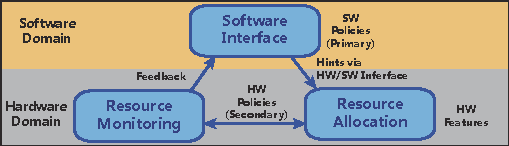
\includegraphics{x86eval/intel-rdt-overview}
  \caption{Intel Resource Director Technology (RDT) 技术示意图}
  \label{fig:intel-rdt-overview}
\end{figure}


CMT and MBM\ref{fig:intel-cmt-flow}
CMT and MBM are new features that allows an operating system (OS) or Hypervisor/virtual machine monitor (VMM) to determine the usage of cache and memory bandwidth by applications running on the platform. Use CMT and MBM to do the following:
 - To detect if the platform supports this monitoring capabilities (via CPUID).  
 - For an OS or VMM to assign an ID for each of applications or VMs that are scheduled to run on a core. This ID is called the Resource Monitoring ID (RMID).      
 - To monitor cache occupancy and memory bandwidth on a per-RMID basis.
 - For an OS or VMM to read LLC occupancy and memory bandwidth for a given RMID at any time.  
 
% Intel CMT Flow
\begin{figure}[H]
  \centering
  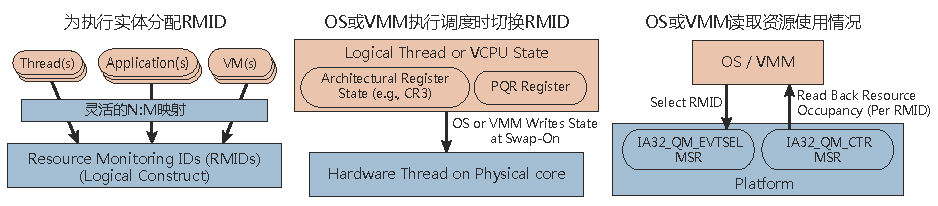
\includegraphics{x86eval/intel-cmt-flow}
  \caption{Intel Cache Monitor Technology (CMT) 技术示意图}
  \label{fig:intel-cmt-flow}
\end{figure}

CAT and CDP
CAT and CDP are new features that allows an OS or Hypervisor/VMM to control allocation of CPU’s shared last level cache. Once CAT or CDP is configured, the processor allows access to portions of the cache according to the established class of service (COS). The processor obeys the COS rules when it runs an application thread or application process. This can be accomplished by performing these steps:
 - Determine if the CPU supports the CAT and CDP feature.
   - The CAT is supported on the following 6 SKUs for Intel(R) Xeon(R) processor E5 v3 family: E5-2658 v3, E5-2658A v3, E5-2648L v3, E5-2628L v3, E5-2618L v3, and E5-2608L v3 and all Intel(R) Xeon(R) processor D SKUs.
 - Configure the COS to define the amount of resources (cache space) available. This configuration is at the processor level and is common to all logical processors.
 - Associate each logical processor with an available COS.
 - Run the application on the logical processor that uses the desired COS

\begin{figure}[H]
  \centering
  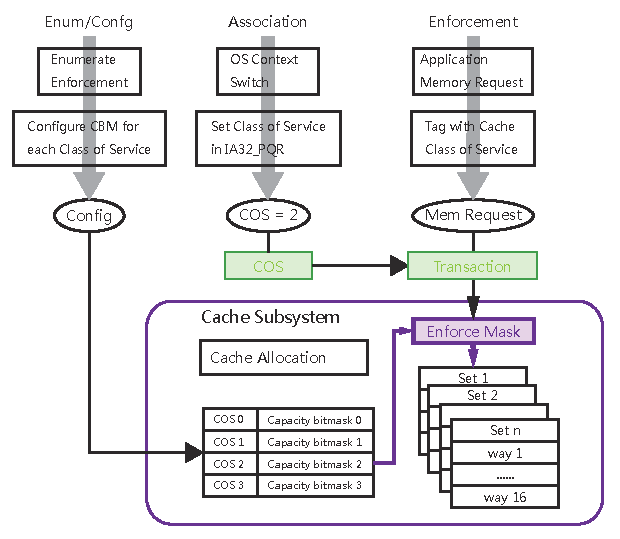
\includegraphics[height=8cm]{x86eval/intel-cat-flow}
  \caption{Intel Cache Allocation Technology (CAT) 技术示意图}
  \label{fig:intel-cat-flow}
\end{figure}

A mechanism \ref{fig:intel-cat-flow} for the OS or Hypervisor to indicate a software-defined ID for each of the software threads (applications,
virtual machines, etc.) that are scheduled to run on a logical processor. These identifiers are known as
Resource Monitoring IDs (RMIDs).

Mechanisms in hardware to monitor cache occupancy and bandwidth statistics as applicable to a given product
generation on a per software-id basis.

Mechanisms for the OS or Hypervisor to signal the Class of Service to which an application belongs, and

Hardware mechanisms to guide the LLC fill policy when an application has been designated to belong to a
specific Class of Service.

\subsubsection*{ARM: Cache partition技术}

该部分需要更多的信息,如ARM64的支持。



\section{共享缓存分析}

\subsection{缓存容量对性能影响}

递减Cache Way,对比性能,找出临界值

\subsection{缓存干扰对性能影响}

1. 运行两个应用,对比在线应用性能变化
2. 采用“限制离线应用缓存占用”策略
3. 采用“隔离在线离线应用缓存”策略

\subsection{小结}

\section{访存带宽分析}

\section{动态资源分配策略}

通过软件监控并设定阈值,对资源进行重新分配。包括Cache、CPU share等

设置不同的监控粒度,对比开销+性能变化



\section{本章小结}

通过本章研究,我们发现在没有体系结构支持的情况下,共享会存在很强烈的干扰现象,在使用
的软件隔离机制(cgroup)或调度机制后,可以在一定程度上缓解干扰。在传统体系结构下进行
扩展的新技术(如CMT/CAT),可以为共享提供一定的保障,但是需要OS或软件提供相应的支持,
因为我们需要一个新的体系结构来实现更好的服务质量保障。



在第\chapterref{cha:intro}章中我们学习了贝叶斯公式~(\ref{equ:chap1:bayes}),这里我们复


在第\chapterref{cha:intro}章中我们学习了贝叶斯公式~(\ref{equ:chap1:bayes}),这里我们复
习一下:
\begin{equation}
\label{equ:chap2:bayes}
p(y|\mathbf{x}) = \frac{p(\mathbf{x},y)}{p(\mathbf{x})}=
\frac{p(\mathbf{x}|y)p(y)}{p(\mathbf{x})} 
\end{equation}



\subsection{绘图}
\label{sec:draw}

本模板不再预先装载任何绘图包(如 \textsf{pstricks,pgf} 等),完全由你自己来决定。
个人觉得 \textsf{pgf} 不错,不依赖于 Postscript。此外还有很多针对 \LaTeX{} 的
 GUI 作图工具,如 XFig(jFig), WinFig, Tpx, Ipe, Dia, Inkscape, LaTeXPiX,
jPicEdt, jaxdraw 等等。

\subsection{插图}
\label{sec:graphs}

强烈推荐《\LaTeXe 插图指南》!关于子图形的使用细节请参看 \textsf{subcaption} 宏包的说明文档。

\subsubsection{一个图形}
\label{sec:onefig}
一般图形都是处在浮动环境中。之所以称为浮动是指最终排版效果图形的位置不一定与源文
件中的位置对应\footnote{This is not a bug, but a feature of \LaTeX!},这也是刚使
用 \LaTeX{} 同学可能遇到的问题。如果要强制固定浮动图形的位置,请使用 \textsf{float} 宏包,
它提供了 \texttt{[H]} 参数,比如图~\ref{fig:xfig1}。
\begin{figure}[H] % use float package if you want it here
  \centering
  
\includegraphics{hello}
  \caption{利用 Xfig 制图}
  \label{fig:xfig1}
\end{figure}

大学之道,在明明德,在亲民,在止于至善。知止而后有定;定而后能静;静而后能安;安
而后能虑;虑而后能得。物有本末,事有终始。知所先后,则近道矣。古之欲明明德于天
下者,先治其国;欲治其国者,先齐其家;欲齐其家者,先修其身;欲修其身者,先正其心;
欲正其心者,先诚其意;欲诚其意者,先致其知;致知在格物。物格而后知至;知至而后
意诚;意诚而后心正;心正而后身 修;身修而后家齐;家齐而后国治;国治而后天下
平。自天子以至于庶人,壹是皆以修身为本。其本乱而未治者 否矣。其所厚者薄,而其所
薄者厚,未之有也!

\hfill ——《大学》


\subsubsection{多个图形}
\label{sec:multifig}

如果多个图形相互独立,并不共用一个图形计数器,那么用 \verb|minipage| 或者
\verb|parbox| 就可以。否则,请参看图~\ref{fig:big1-subcaptionbox},它包含两个小图,分别是图~\ref{fig:subfig1} 
和图~\ref{fig:subfig2}。推荐使用\verb|\subcaptionbox|,
因为可以像图~\ref{fig:big1-subcaptionbox} 那样对齐子图的标题,
也可以使用\textsf{subcaption}宏包的\verb|\subcaption|(放在minipage中,用法同\verb|\caption|)
或是 subfigure 、 subtable环境,像图~\ref{fig:big1-subfigure},不要再用 \verb|\subfloat|、
\verb|\subfigure| 和 \verb|\subtable|。
\begin{figure}[h]
  \centering%
  \subcaptionbox{第一个小图形\label{fig:subfig1}}
  [3cm] %标题的长度,超过则会换行,如下一个小图。
    {
\includegraphics[height=3cm]{thu-fig-logo}}
      \hspace{4em}%
  \subcaptionbox{第二个小图形,注意这个图略矮些。如果标题很长的话,它会自动换行\label{fig:subfig2}}
      {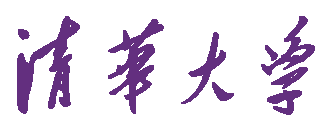
\includegraphics[height=2cm]{thu-text-logo}}
  \caption{包含子图形的大图形(subcaptionbox示例)}
  \label{fig:big1-subcaptionbox}
\end{figure}
\begin{figure}[h]
  \centering%
  \begin{subfigure}{3cm}
    
\includegraphics[height=3cm]{thu-fig-logo}
    \caption{第一个小图形}
  \end{subfigure}
  \hspace{4em}%
  \begin{subfigure}{0.5\textwidth}
    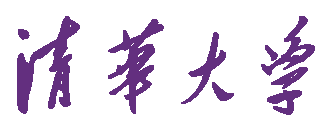
\includegraphics[height=2cm]{thu-text-logo}
    \caption{第二个小图形,注意这个图略矮些。subfigure中同一行的子图在顶端对齐。}
  \end{subfigure}
  \caption{包含子图形的大图形(subfigure示例)}
  \label{fig:big1-subfigure}
\end{figure}
古之学者必有师。师者,所以传道受业解惑也。人非生而知之者,孰能无惑?惑而不从师,
其为惑也,终不解矣。生乎吾前,其闻道也固先乎吾,吾从而师之;生乎吾後,其闻道也亦
先乎吾,吾从而师之。吾师道也,夫庸知其年之先後生於吾乎!是故无贵无贱无长无少,道
之所存,师之所存也。

嗟乎!师道之不传也久矣,欲人之无惑也难矣。古之圣人,其出人也远矣,犹且从师而问焉;
今之众人,其下圣人也亦远矣,而耻学於师。是故圣益圣,愚益愚。圣人之所以为圣,愚
人之所以为愚,其皆出於此乎?爱其子,择师而教之,於其身也,则耻师焉,惑焉。彼童子
之师,授之书而习其句读者,非吾所谓传其道、解其惑者也。句读之不知,惑之不解,或师
焉,或不焉,小学而大遗,吾未见其明也。巫医、乐师、百工之人不耻相师,  士大夫之族
曰“师”曰“弟子”之云者,则群聚而笑之。问之,则曰:彼与彼年相若也,道相似也,位
卑则足羞,官盛则近谀。呜呼!师道之不复,可知矣。巫医、乐师、百工之人。吾子不齿,
今其智乃反不能及,其可怪也欤!圣人无常师。孔子师郯子、苌子、师襄、老聃。郯子之徒,
其贤不及孔子。孔子曰:“三人行,必有我师。”是故弟子不必不如师,师不必贤於弟子。
闻道有先後,术业有专攻,如是而已。

如果要把编号的两个图形并排,那么小页就非常有用了:
\begin{figure}
\begin{minipage}{0.48\textwidth}
  \centering
  
\includegraphics[height=2cm]{thu-whole-logo}
  \caption{并排第一个图}
  \label{fig:parallel1}
\end{minipage}\hfill
\begin{minipage}{0.48\textwidth}
  \centering
  
\includegraphics[height=2cm]{thu-whole-logo}
  \caption{并排第二个图}
  \label{fig:parallel2}
\end{minipage}
\end{figure}

李氏子蟠,年十七,好古文、六艺,经传皆通习之,不拘於时,学於余。余嘉其能行古
道,作师说以贻之。

\hfill —— 韩愈(唐)

